\renewcommand*{\arraystretch}{1.1}

\subsection*{BI / read / 24}
\label{sec:bi-read-24}

\noindent\begin{tabularx}{\queryCardWidth}{|>{\queryPropertyCell}p{\queryPropertyCellWidth}|X|}
	\hline
	query & BI / read / 24 \\ \hline
%
	title & Messages by Topic and Continent
 \\ \hline
%
	pattern & \hfill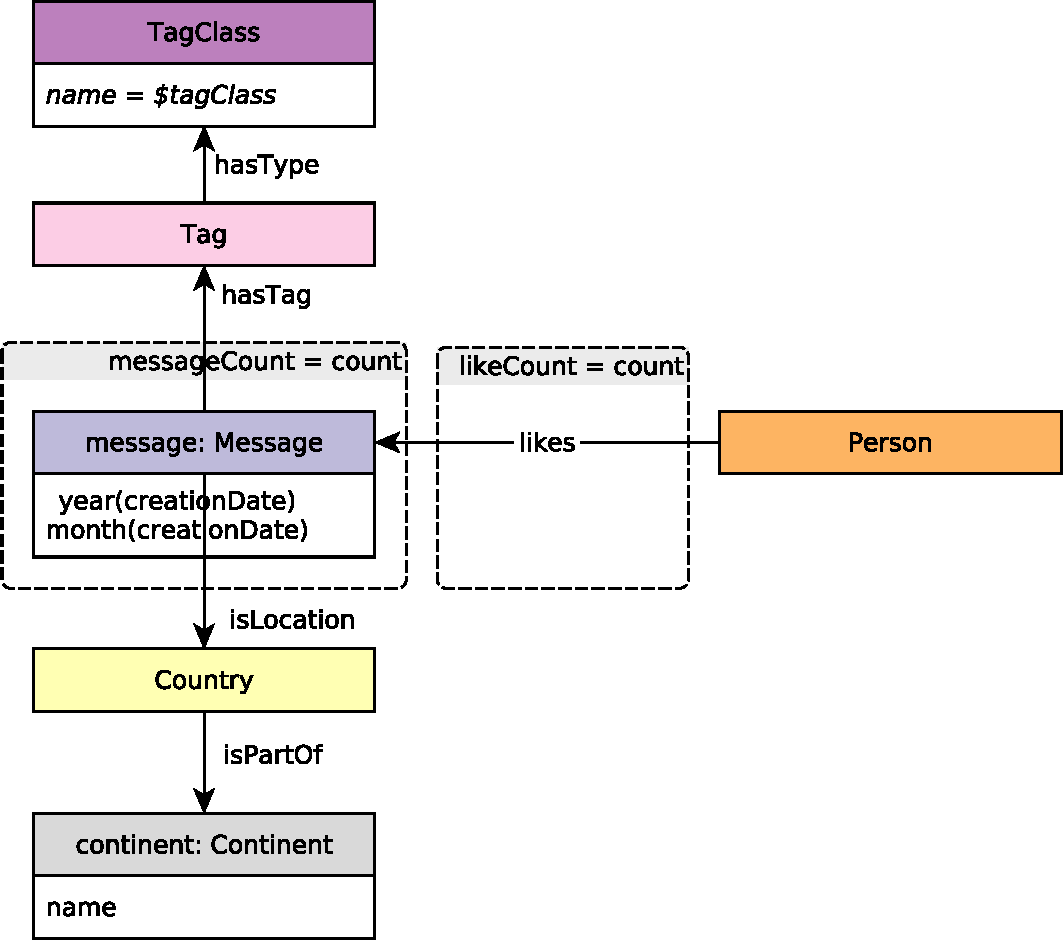
\includegraphics[scale=\patternscale,margin=0cm .2cm]{patterns/bi-read-24}\hfill\vadjust{} \\ \hline
%
	desc. & Find all Messages tagged with a Tag from the given TagClass
(non-transitive).

Count all Messages and their likes grouped by continent, year, and
month.
 \\ \hline
%
	
		group by &
		\multicolumn{1}{>{\raggedright}X|}{
			\varNameText year
, 
			\varNameText month
, 
			\varNameText continent.name

			} \\ \hline
	
%
	
		params &
		\innerCardVSpace{\begin{tabularx}{\attributeCardWidth}{|>{\paramNumberCell}c|>{\varNameCell}M|>{\typeCell}m{\typeWidth}|Y|} \hline
		$\mathsf{1}$ & tagClass
 & String
 &  \\ \hline
		\end{tabularx}}\innerCardVSpace \\ \hline
	
%
	
		result &
		\innerCardVSpace{\begin{tabularx}{\attributeCardWidth}{|>{\resultNumberCell}c|>{\varNameCell}M|>{\typeCell}m{\typeWidth}|>{\resultOriginCell}c|Y|} \hline
		$\mathsf{1}$ & messageCount
 & 32-bit Integer
 & R &
				 \\ \hline
		$\mathsf{2}$ & likeCount
 & 32-bit Integer
 & R &
				 \\ \hline
		$\mathsf{3}$ & year
 & 32-bit Integer
 & R &
				year of the Message's creationDate
 \\ \hline
		$\mathsf{4}$ & month
 & 32-bit Integer
 & R &
				month of the Message's creationDate
 \\ \hline
		$\mathsf{5}$ & continent.name
 & String
 & R &
				 \\ \hline
		\end{tabularx}}\innerCardVSpace \\ \hline
	
%
	
		sort		&
		\innerCardVSpace{\begin{tabular}{|>{\sortNumberCell}c|>{\varNameCell}l|>{\directionCell}c|} \hline
		$\mathsf{1}$ & year
 & $\asc
$ \\ \hline
		$\mathsf{2}$ & month
 & $\asc
$ \\ \hline
		$\mathsf{3}$ & continent.name
 & $\desc
$ \\ \hline
		\end{tabular}}\innerCardVSpace \\ \hline
	%
	limit & 100 \\ \hline
	%
	CPs &
	\multicolumn{1}{>{\raggedright}l|}{
		\chokePoint{1.6}, 
		\chokePoint{2.1}, 
		\chokePoint{2.3}, 
		\chokePoint{2.4}, 
		\chokePoint{3.2}, 
		\chokePoint{4.3}
		} \\ \hline
	%
	%
\end{tabularx}
\queryCardVSpace